\documentclass[conference,9pt,letterpaper]{IEEEtran}
\usepackage{amsmath,amssymb,graphicx,booktabs,array,fontspec,unicode-math}
\setmainfont{NotoSerifCJKsc-Regular.otf}[BoldFont=NotoSerifCJKsc-Bold.otf]
\setsansfont{NotoSansCJKsc-Regular.otf}[BoldFont=NotoSansCJKsc-Bold.otf]
\setmathfont{Latin Modern Math}
\XeTeXlinebreaklocale "zh"
\XeTeXlinebreakskip=0pt plus 1pt
\setlength{\dbltextfloatsep}{8pt plus 2pt minus 2pt}
\usepackage[hidelinks]{hyperref}
\hypersetup{pdftitle={LoDA-SA：低频距离感知稀疏注意力},pdfauthor={},pdfcreator={LaTeX}}
\graphicspath{{../figures/}}
\newcommand{\Top}{\operatorname{TopK}}
\renewcommand{\abstractname}{摘要}
\renewcommand{\figurename}{图}
\renewcommand{\tablename}{表}
\title{LoDA-SA：低频距离感知稀疏注意力}
\author{\IEEEauthorblockN{匿名作者}}
\begin{document}
\maketitle
\begin{abstract}
有限候选预算需要为不同位置区域保留有用历史的访问机会，同时避免选择成本超过省去的注意力计算。本文研究LoDA-SA，即低频距离感知稀疏注意力，采用页到词元的两级级联。LoDA-SA先明确距离区域的候选准入：$n_l$定义近区，$n_b$预留其L1页数，远区使用剩余页预算；共享32个低频RoPE坐标缩窄两级评分点积。两区候选页与非对齐保护边界页共同进入一次L2词元竞争，再计算原维注意力。4个前缀词元和近期窗口另行保护。Qwen3诊断促使我们考察区域准入，但未证明混合评分优势：固定预算下最佳所测混合方案平均漏失为.135，全局极值为.121。历史任务比较使用不同词元分配，独立计时还显示稀疏解码更慢；两者均不验证当前LoDA-SA。仍需匹配质量与包含准备开销的完整请求测量。

\end{abstract}
\begin{IEEEkeywords}稀疏注意力，共享表示，区域检索，长上下文推理\end{IEEEkeywords}

\section{引言}
长上下文解码需要在有限注意力预算下保留对有用历史的访问。不同距离的词元竞争同一预算，而全局排名本身不为某个位置区域预留候选入口。因此，距离可以用来组织选择，但不意味着重要性随距离单调下降，也不意味着近处词元总是更重要。选择器需要先明确哪些区域能够提供候选，再以足够低的成本排序，使限制最终注意力支持集具有意义。

AsyncTLS等级联使用低成本页摘要筛选候选页，再进行词元精筛~\cite{asynctls}。均值池化与符号感知极值都不按页内注意力权重总和排序，本文的选择器也采用这两类摘要。沿用ClusterKV的词元／页分析视角~\cite{clusterkv}，图\ref{fig:observation}(a)中的单个Qwen3查询显示：按注意力权重总和排序的参考页漏选更少时，漏失的参考页权重反而更多。由于区域分配与实际词元数不同，这一诊断不是受控比较，但促使我们考察评分与预算如何共同影响候选进入后续筛选的机会。

在四条序列的128条相关观测中，两种全局选择器呈现不同的区域漏失质量构成（图\ref{fig:observation}(b)）。以每条查询的质量排序参考集总质量归一化后，block-avg的近区／远区平均漏失份额为.084／.170，符号感知极值为.079／.042。极值摘要在两区的平均漏失均较低；这些诊断不能证明区域分工或近区等价。在固定2048词元上限下，所测23种near-avg／far-extrema配额拆分中，最佳平均漏失为.135，全局极值为.121。这一有界诊断扫描既未建立混合方案优势，也未建立任务质量收益。

本文围绕LoDA-SA（低频距离感知稀疏注意力）组织设计。距离感知策略以$n_l$指定近区范围、$n_b$指定近区页预算，其余L1预算分配给远区；这控制的是区域候选准入，而非最终近远词元份额。两级随后共用32个坐标，即16个完整低频RoPE旋转对；L2对合并候选做一次TopK，再用原始全维Q/K/V计算注意力。图\ref{fig:observation}(c)中，低频配对平均保留全维参考mid-TopK权重和的.84，随机坐标为.51，高频配对为.24；随机32未配对。这些诊断不能证明任务质量保持。叙述从距离策略展开，实际执行则先准备共享表示，再进行区域选择。普通L2仍在掩码前评分完整历史，历史可选门控保持关闭。

LoDA-SA在已有两级选择范式内研究显式距离区域页预算、共享低频评分视图与统一词元竞争的组合。贡献是这一组合的机制说明及有界证据，不是首次提出页到词元级联，也不是已验证的质量--时延提升。历史预算耦合分析区分页准入与最终词元覆盖；历史任务比较和更慢的稀疏解码共同限制结论。当前方法仍需匹配质量及包含准备、维护和选择开销的完整请求成本评估。

\begin{figure*}[t]\centering
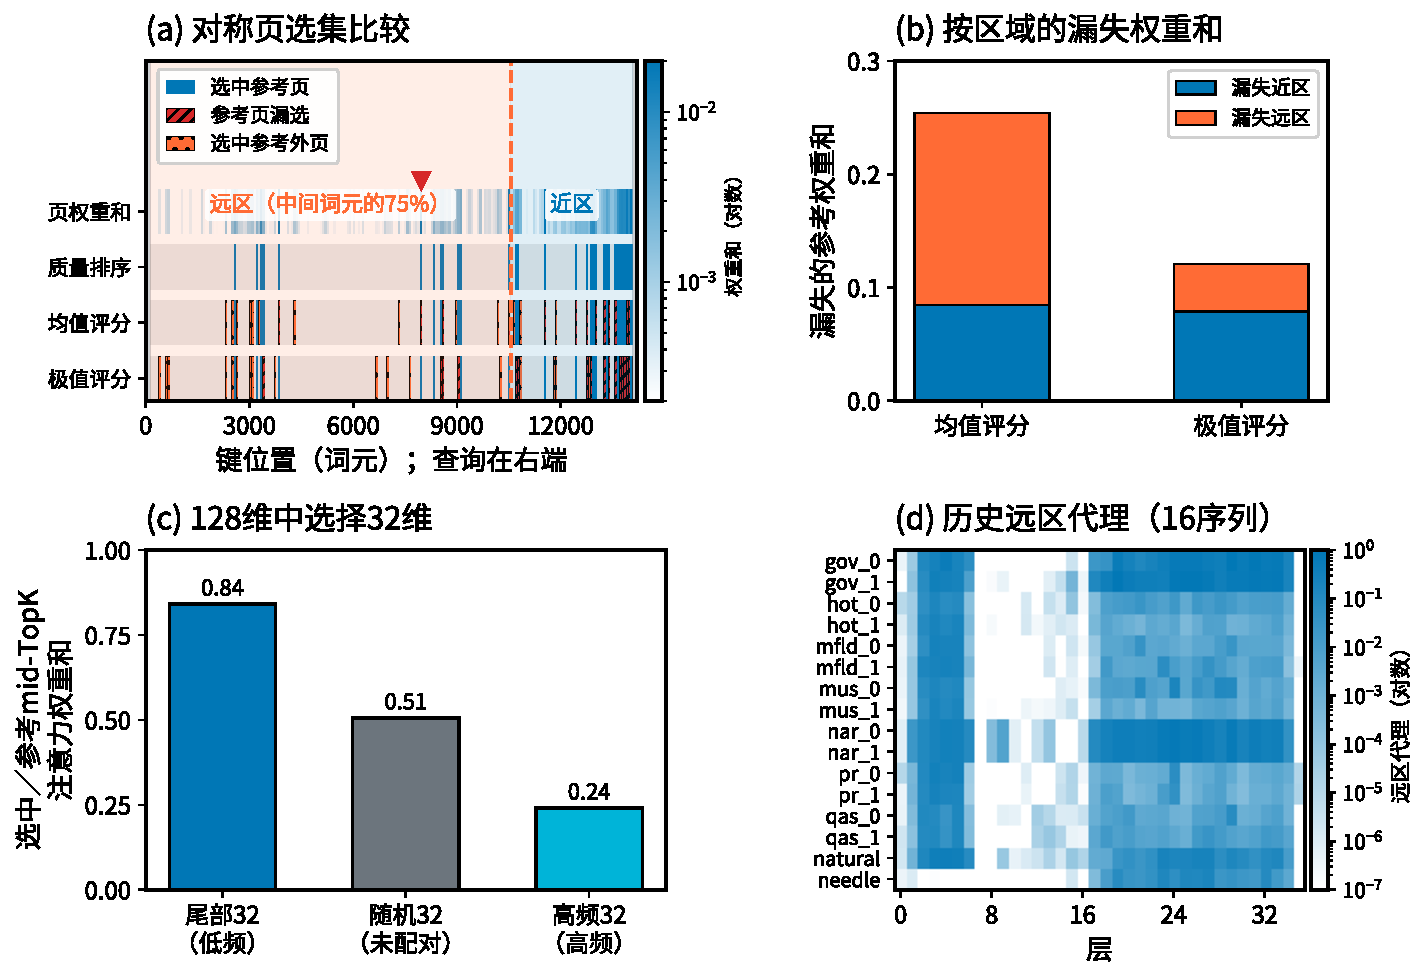
\includegraphics[width=\textwidth]{o_observation_zh.pdf}
\caption{LoDA-SA的设计动机诊断，模型为Qwen3-8B；(a)--(c)前缀／近期保护各128。(a) MuSiQue样本1、层24、查询14212。顶行是逐页注意力权重和，不是选集；下三行为注意力权重排序参考、均值与极值选集，均32页，在2048上限下实际使用1989/1989/2048词元。均值／极值分别漏选13／17个参考页，其中包含参考页注意力权重总和的59.65\%／26.46\%。蓝色为选中参考页，红色斜线为参考漏页，橙色点纹为参考外入选页。整页注意力权重排序只是比较参考，并非最优oracle、精确词元TopK或DSA；均值与极值共享32坐标及头聚合，参考采用全维注意力权重。实际区域分配和词元数不同，漏页不能证明近远分工或任务质量优劣。(b) 区域漏失参考质量的平均份额：先将每条查询在各区漏失的参考质量除以该查询的质量排序参考集总质量，再对四条序列的128条相关观测求均值。极值摘要在两区的漏失均较低，不能据此证明区域分工。(c) 选中权重和相对全维参考mid-TopK权重和；随机32不保留RoPE配对。(d) 单张16×36历史单查询代理矩阵中，24/36层的中位值低于.01，每序列有12--32个低代理值层；使用最后采样查询、组内logits先求和后softmax及旧远区$[64,t-2048)$，不同于所讨论的历史可选门控统计（S6）。这些选择和统计不构成任务质量或解码安全结果。}
\label{fig:observation}\end{figure*}

\section{相关工作}
Quest提供符号感知页极值界，SparQ从查询选择键坐标，HISA按层级剪枝注意力集合~\cite{quest,sparq,hisa}。AsyncTLS明确在粗粒度选块时沿用Quest，在细粒度选词元时采用Double Sparsity，并结合量化、逐查询归一化与GQA概率聚合及原始KV注意力~\cite{asynctls}；更早的Twilight采用先选择再剪枝架构~\cite{twilight}。LoDA-SA沿用这一广义层级选择范式，研究显式距离区域页准入、两级共享完整低频RoPE对与统一L2竞争的组合。这里陈述的是算法思想关系，不是已核实的直接代码继承。

选择器自身读取什么同样重要。Token-Picker从部分键比特块构造保守概率估计，对被剪枝词元停止后续键比特块和value的传输~\cite{tokenpicker}；本文的选择器则在页与词元预算约束下用固定坐标子集对候选排序，并保留原维KV。本文的bf16配置储存浮点评分键；AsyncTLS使用打包INT4词元级索引，FFD扫描2-bit键缩略表示~\cite{asynctls,ffd}。紧凑坐标与区域配额用于控制评分宽度和候选访问。KV压缩与放置方法关注互补的存储和数据移动约束~\cite{shadowkv,million,clusterkv}；较小的评分视图不减少原始KV容量，也不能据此证明完整请求时延收益。

\section{LoDA-SA：共享子空间中的距离感知选择}
LoDA-SA区分三项决策：哪些距离区域能够提供候选页、如何用共享紧凑视图评分，以及合并候选中的哪些词元进入最终注意力。距离策略用$n_l$指定近区范围、$n_b$指定近区页预算，远区获得$K_1-n_b$页。实现先准备共享32坐标表示，再执行区域L1选择（图\ref{fig:architecture}）；这一执行顺序不同于从距离策略开始的叙述顺序。选择仅在解码阶段执行，预填充保持稠密。参考L2评分全历史，再施加合并页候选掩码并执行一次中间词元TopK；入选索引与保护位置共同定义原维注意力支持集。该参考配置关闭门控与候选收集，归档运行不验证当前LoDA-SA。

\begin{figure*}[t]\centering
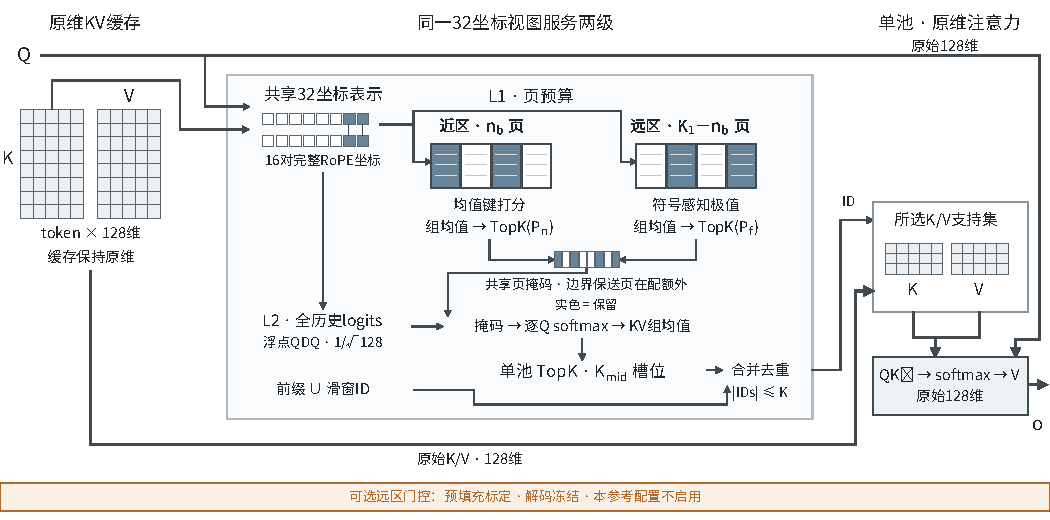
\includegraphics[width=\textwidth]{architecture_domains/fig2_domains_zh.pdf}
\caption{LoDA-SA分区参考架构：边界页保送开启，门控与候选收集关闭。共享坐标表示用于区域L1页评分和普通全历史L2评分。同一时间顺序的页面划分近远；非对齐保护边界页在L1配额之外并入页掩码，只有保护词元绕过最终选择。页掩码限制候选资格；逐查询softmax及KV组概率均值后进行一次合并中间候选的TopK。保护位置与索引合并去重后满足$K$。近区不含保护滑窗。索引定义原维K/V支持集，物理聚集或带掩码稠密计算由后端决定；阵列均为示意。}
\label{fig:architecture}\end{figure*}

\subsection{距离区域与候选预算}
在解码过程中，令$t$表示当前词元在完整序列中从0计数的位置（包含预填充词元）。$s$与$w$分别表示受保护前缀和近期窗口的长度，保护集$\mathcal P_t=\{i:0\le i\le t,\ i<s\ \text{或}\ i>t-w\}$，未保护中间区$\mathcal M_t=\{0,\ldots,t\}\setminus\mathcal P_t$；保护重叠仅计一次。请求的近区长度为$n_l$个词元。实现取至少一页的长度$L=\max(B,n_l)$，再将近远切点向下对齐至页边界；近区结束于保护滑窗起点，远区为其余中间历史。近区不包含受保护的近期窗口。

对普通长历史、保护不重叠且总上限$K\geq|\mathcal P_t|$，定义$K_{\mathrm{mid}}=K-|\mathcal P_t|$。LoDA-SA使用$n_l$和近区页预算$n_b$，远区页预算为$K_1-n_b$；页配额按可用页数截断。近远两区选中页与保护边界保送页共同构成L2候选池，一次TopK在合并候选中使用$K_{\mathrm{mid}}$个槽位。当前不设置近远区域词元配额；最终区域份额由分数竞争决定，而非词元配额。当正概率候选充足时，L2不能恢复被L1排除页中的未保护词元；候选不足与掩码后零值并列的例外见S7。

保护不重叠时，$K=1024$、$s=4$、$w=128$为每个KV头留下名义892个共享中间槽位。部分前缀页可能再次选中保护位置；最终并集会去重，因此不同未保护入选词元数可能更少。页候选资格、最终入选和预算的精确利用率是不同概念。




\subsection{共享低频坐标}
每层、每KV头的两个区域和两个筛选阶段采用相同的坐标映射，各查询头仍独立评分。对Qwen3-8B的尾部坐标配置，从128维RoPE后查询与键中选择$J=\{48,\ldots,63,112,\ldots,127\}$。这些索引保留16个完整的低频split-half RoPE旋转对（补充图S1）；该陈述不泛指全维、静态配对、投影或MLA配置。令$E_J\in\mathbb R^{128\times32}$为坐标选择矩阵，评分向量为$z_q=E_J^\top q$与$z_i=E_J^\top k_i$。所保留旋转对的位置旋转较慢，为这一选择提供动机，但不保证保留重要词元。紧凑实现使用32维评分张量，而历史质量运行在128维L2张量中保留32个有效坐标（S7）。

L1将选定的键坐标聚合为页摘要，用于粗粒度排序；L2在同一坐标视图中用逐词元分数精筛。两种评分视图分别存储。原始键和值仍保持全维。紧凑实现将每次评分点积缩窄至四分之一，但辅助视图的准备与维护增加工作，并未压缩原始KV缓存（S7）。



\subsection{区域页评分与边界候选资格}
级联设置区域页上限与一个共享词元预算（补充图S2）。近区页采用查询与平均键的点积汇总页级相关性；远区页采用符号感知极值来上界共享空间词元分数，这一区域分工属于评分启发式。页摘要覆盖完整物理页，包括保护位置（S7）。在分区路径中，若前缀结束或保护滑窗起点位于页内，该边界页会绕过L1排名：先从竞争池移除，再额外并入候选，不占区域页配额。页内未保护词元仍须参与L2竞争；只有保护词元强制进入最终支持集。近远分界按页对齐，不额外触发保送。对这样的非空页$b$，定义$m_{b,j}=\min_{i\in b}z_{i,j}$与$M_{b,j}=\max_{i\in b}z_{i,j}$。Quest极值构造~\cite{quest}给出
\begin{equation}
U_b(z_q)=\sum_j(z_{q,j}^{+}M_{b,j}+z_{q,j}^{-}m_{b,j}),
\end{equation}
其中$z^+=\max(z,0)$、$z^-=\min(z,0)$。对页$b$中所表示的每个共享空间键$z_i$，都有$z_q^\top z_i\leq U_b(z_q)$，因为每个带符号坐标项均由所选极值上界。这不构成对原维logits的相应保证。由于各坐标极值可能来自不同词元，$U_b$可能高估页内所有词元的分数，因此只保留评分最高的页仍可能漏掉重要词元。平均键页评分不提供这一逐词元上界。


\subsection{GQA聚合与原维注意力}
GQA将32个查询头按每个KV组4个分到8个KV头。L1对组内查询的页分数取平均再做区域TopK。普通L2先为每个查询计算全历史词元logits，施加共同的保留页掩码，并在该支持集上归一化；随后在KV组内对概率取均值，再对合并中间候选进行一次TopK。在该Qwen3实现中，L2 logits在逐查询softmax前仍使用原始头维度对应的$1/\sqrt{128}$缩放，包括采用32个坐标评分的情形。由于先逐查询softmax再做组内平均，该规则通常不同于对组内平均logits施加softmax。更小的L1候选页集合缩小的是候选资格范围，而非普通L2沿全历史的词元点积数量。

对KV组$h$，令$\mathcal S_{t,h}$为保护位置与统一竞争入选词元索引的去重并集，并满足$|\mathcal S_{t,h}|\leq K$。组内各查询$g$使用相同词元索引，但以头维度$d=128$独立重算原维注意力：
\begin{equation}
o_{h,g}=\sum_{i\in\mathcal S_{t,h}}\frac{e^{q_{h,g}^{\top}k_{i,h}/\sqrt d}}{\sum_{j\in\mathcal S_{t,h}}e^{q_{h,g}^{\top}k_{j,h}/\sqrt d}}v_{i,h}.
\end{equation}
每个查询在合并后的索引上统一施加softmax，而非直接相加各区域独立归一化的输出~\cite{salo}。保留词元的Q/K logits采用原维计算，但缩小支持集会改变分母，并可能改变注意力输出。这些索引定义共同的逻辑支持集；KV的物理聚集与复用取决于后端和序列长度，短序列可使用带掩码的稠密路径。

\subsection{可选远区门控的适用范围}
当前$n_l/n_b$设计关闭远区门控。历史扩展在逐头因果softmax后，以末尾预填充查询的远区质量标定层决策，并在稀疏解码时冻结。其数值词元配额分支可以回填近区词元配额，但这不是当前统一L2规则（S5）。在统一分支中，移除普通远区页竞争并不保证最终远区词元全部消失：前缀边界页仍可能进入合并竞争。因此本文不宣称完整跳过远区，也不将历史门控结果移用于当前设计。标定阈值不约束解码误差，质量与完整请求成本均需另行评估。

\begin{figure*}[t]\centering
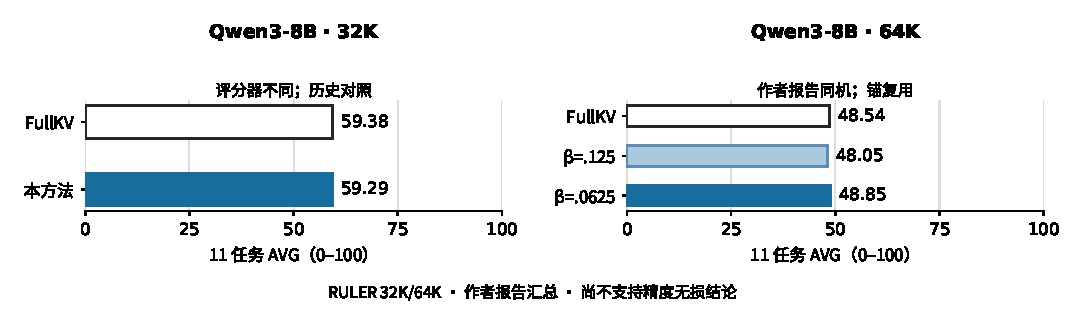
\includegraphics[width=\textwidth]{ruler32k_comparison/ruler32k_avg_compact_zh.pdf}
\caption{作者报告的Qwen3-8B RULER 32K/64K结果：11任务算术AVG，每任务每臂100例。FullKV为稠密参照；稀疏臂报告$K=1024$、4/128保护。这些历史数值词元配额臂不评测当前统一L2设计。32K面板展示近区配额(8,320)，64K展示(8,320)与(16,640)。32K比较跨机器且评分器不同；64K稀疏两臂报告同机，FullKV锚来自另次运行。门控状态和实际评分维数未核。描述性得分不构成非劣性或匹配质量--成本收益（S8）。}
\label{fig:ruler32k-quality}\end{figure*}

\section{实验设置}
本文分别考察任务质量（Q1）、区域候选覆盖（Q2）与执行成本（Q3）。表\ref{tab:settings}给出面向Qwen3-8B的LoDA-SA设计：稠密预填充、稀疏解码、显式$n_l/n_b$页选择及统一L2；1024词元上限包含4个前缀与128个近期词元。当前方法不调节$\alpha$、$\beta$、$\gamma$或近区词元配额；下述记录尚不能建立该配置的匹配完整运行。历史数值词元配额运行保留原身份；$(8,320)$表示近区页数和词元数，不是$(n_l,n_b)$。历史LongBench采用128/128保护、128维L2键中的32个有效坐标及16级量化--反量化（S7）。名义全维页／词元变体缺少完整执行配置，不构成受控单阶段消融；选择器与解码计时来自未匹配质量和成本的独立研究。

\begin{table}[t]\centering\small
\caption{紧凑设计的参数与执行策略。显式$n_l,n_b$数值为配置参数，不是此处已验证的测量。$K$包含去重保护词元。}\label{tab:settings}
\begin{tabular}{ll}\hline
参数 & 设置 \\\hline
最终词元上限$K$ & 1024\\
页长；L1页上限$K_1$ & 64；128\\
近区页预算（远区） & $n_b$（$K_1-n_b$）\\
L2中间词元选择 & 一次合并TopK\\
近区范围 & $n_l$词元；切点按页对齐\\
L1/L2有效坐标 & 32/32\\
前缀／近期保护 & 4/128\\
预填充；解码层 & 稠密；全层稀疏\\\hline
\end{tabular}\end{table}

\textbf{工作负载与对照。}作者报告的质量记录覆盖五项LongBench任务（问答、摘要与代码补全）~\cite{longbench}，以及Qwen3-8B在32K／64K和历史128K上的11任务RULER~\cite{ruler}集合，另含移植的Quest/AsyncTLS/JSSA基线。LongBench的三种名义稀疏变体不构成已验证的完整双因素消融；FullKV是RULER与解码计时中的稠密参照，不设稀疏词元上限。原生方法比较要求保留并披露各方法的预填充／解码路径；统一阶段策略后的适配结果须单独报告。预算匹配须对齐含保护位置的最终去重词元上限$K$；实际选集大小与头间共享粒度影响KV流量，仅匹配$K$既不能证明质量相同，也不能建立成本匹配比较（S7）。

\textbf{指标。}主要质量指标为每项基准与长度比较中固定任务集合上各任务得分AVG；逐任务增减用于解释AVG，不要求每项任务均零掉分。阶段策略匹配的受控比较须匹配模型、样本、长度、评分器与阶段策略并对齐词元预算；未完成的集合不构成完整集合的AVG。图\ref{fig:observation}(b)先以每条查询的参考集总质量归一化区域漏失质量，再对相关观测取均值；图\ref{fig:observation}(c)则以全维参考mid-TopK权重和为分母。选择器时间（合成单层）与同步TPOT（首输出后的模型级生成间隔）均不测量计入准备、维护及输入输出工作的完整请求时延。未配对的质量与计时研究不能定义质量--时延前沿；AVG差异属于描述性比较，不构成统计非劣性证据。

\begin{figure}[t]\centering
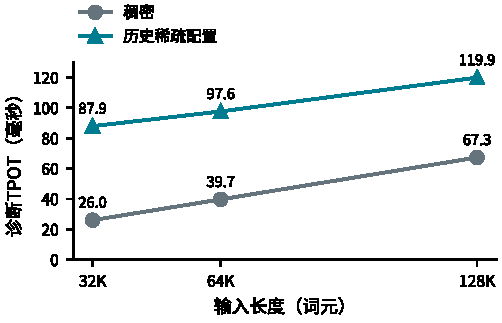
\includegraphics[width=\columnwidth]{decode_tpot_current_zh.pdf}
\caption{作者报告的历史稀疏配置与稠密FullKV模型级解码TPOT，采用Qwen3-8B及动态缓存。固定输出128词元，对应127个首输出后间隔，包含设备同步与argmax。历史$(.125,.375,.625)$设置不同于当前$n_l/n_b$设计；这些中位数不测量完整请求E2E，也不建立匹配质量--成本比较（S6）。}
\label{fig:pending-evaluation}\end{figure}

\section{评估与讨论}
\subsection{Q1：缩小评分宽度能否保留任务质量？}
在HotpotQA、Qasper、MuSiQue、GovReport和RepoBench-P~\cite{longbench}上，五项任务均值在三种名义评分配置间的差距不超过0.33分：共享子空间评分平均分为47.588，名义全维页评分与词元评分变体分别为47.910和47.666（补充图S4），共享子空间臂分别比两变体低0.322与0.078分。这些差值描述已记录配置，并非缩小评分宽度保持质量的证据：变体未被确认为单因素干预，共享子空间运行也采用较早的128/128保护实现。三者均为稀疏配置，稠密FullKV是另一类参照。

\subsection{Q2：区域预算如何约束候选访问？}
本节比较保留历史数值词元配额身份，不验证当前$n_l/n_b$取值。图\ref{fig:observation}(b)展示全局选择器的区域漏失构成，并非区域配额收益；固定总上限的混合扫描同样保留负例（.135对.121）。作者报告的8B 32K研究中，在$K_1=128$、$K=1024$、4/128保护下，近区配额$(16,640)\rightarrow(8,320)$（归档$\beta=.125\!\rightarrow\!.0625$）使AVG从58.30变为59.29；远区页由112增至120、远区词元预算由252升至572，同时改变。归档$\beta=.03125$下，$K_1=128$得58.07，近区页为4、远区词元预算为732；$K_1=256$得58.96，近区配额$(8,320)$与59.29分臂相同，但远区页由120扩至248。两臂均低于59.29；相对59.29分臂，$K_1=256$臂的CWE升3.9分、FWE降9.67分。这些稀疏臂的数据／评分器记录匹配，但预测未独立重放。

\textbf{历史比例耦合。}早期运行按$n_p=\max(1,\operatorname{round}(\beta K_1))$与$n_k=\min(\lfloor\gamma n_pB\rfloor,K_{\mathrm{mid}})$派生配额，半整数取偶，其名义远区预算为
\begin{equation}
k_f=K_{\mathrm{mid}}-\min(\lfloor\gamma n_pB\rfloor,K_{\mathrm{mid}}).
\label{eq:coupling}
\end{equation}
这是历史数值词元配额规则，不是当前统一L2算法。

\textbf{隐式耦合失效。}归档诊断展示了式\eqref{eq:coupling}的全部三种重分配。对归档公式做整数枚举，$K=1024$（$B=64$、$\beta=.125$、$\gamma=.625$、128/128保护）下首个远区归零的页上限为$K_1=156$，$K_1=155$时远区预算尚余8：容量看似随$K_1$增长而远区词元消失。归档任务扫描中，HotpotQA恰在远区预算为零的臂上从53.6--57.3塌缩到37.7，损伤按远区占比分级（占比.875时16.4分，.125时约1分）。在归档网格点$(\alpha,\beta)=(.25,.125)$，自由竞争与最优$\gamma$在保留质量诊断中相差不超过.001（两者均约.852），而$\gamma=0$读作“无远区保留”，实际将近区词元配额压为零，保留质量降至.827。历史128K RULER臂按其报告预算推得$k_f=0$（S6）。这些归档诊断统一了三种异常，但不是新的受控实验。

作者报告的Qwen3-8B 32K相对稠密FullKV的AVG差值为$-0.09$分，比较跨机且评分协议不同。64K下，8B近区配额(8,320)/(16,640)两臂AVG为48.85/48.05，另一次运行的稠密锚为48.54。稀疏两臂同机且评分器相同，但预测协议不同；稠密对照也采用不同评分器。这些描述性比较不能建立因果或统计非劣结论（S8）。

\textbf{移植基线比较。}名义预算为512时，作者报告本选择器AVG为56.00、AsyncTLS为48.33（报告值相差7.67分）。最终去重词元预算、保护策略与执行阶段尚未匹配（S8）。$K=1024$时AVG为59.29，对照JSSA的58.7（名义预算1024）、Quest的42.85与FASA的18.64；$K=384$得15.00。移植出处、CWE的43.4分下降及缺失的配对区间见S8。

128K下，同机稀疏两臂分别得45.73（(8,320)）和46.02（(16,640)）；前者为另次运行稠密锚46.43的98.49\%。历史128K RULER报告稀疏臂得分23.98，报告预算推得保留远区页时$k_f=0$，执行未验证、22.45分损失未解释（S6）。另一组五任务LongBench比较中，仅保护词元的平均分为26.09，复用的稀疏检索参照为47.91；两者预算分别为256和1024词元，因此检索与预算同时变化。

\subsection{Q3：紧凑评分能否降低执行成本？}
\textbf{模型级解码。}在每个测量长度上，所报告的稀疏配置均慢于稠密FullKV（图\ref{fig:pending-evaluation}）。32K、64K与128K下，稀疏TPOT中位数为87.9、97.6和119.9毫秒，稠密为26.0、39.7和67.3毫秒。相对代价随长度减小，但稀疏TPOT绝对值仍增加：无解码时间收益。计时包含设备同步与argmax，配置不同于紧凑设计，汇总中位数不能定位原因，也不能预测紧凑实现的性能（S6）。

\textbf{选择器局部成本。}一项独立的两轮合成实验（单层、批量大小为1、单查询、64K长度QKV）给出稳态汇总：名义全维页评分1.3502毫秒，共享子空间评分1.3598毫秒，名义全维词元评分1.4634毫秒；共享子空间第一轮慢0.0237毫秒、第二轮快0.0046毫秒。原始采样序列缺失且采样协议差异尚未解决，无法可靠评估这些小幅差异（S6）。这些局部计时不能定位瓶颈，未与质量评估配对，也未测量完整请求成本。

\subsection{可选门控：预填充不保证解码需求}
低预填充注意力并不能证明解码时可安全跳过远区选择。一条归档输入--层记录的预填充远区注意力代理量低于.05，而所报告的解码尾部五个查询均值为.1678：这是代理量跨阶段变化，并非测得的任务质量损失。门控阈值.05和.10对应五任务AVG为47.876和47.692，相对复用的47.910参考分别下降.034和.218分，每臂仍有三项任务下降，其中HotpotQA分别下降1.05和1.26分；AVG仍是主判据，不设逐任务零损门槛。小幅AVG变化或包含零的任务自助法区间均不能证明统计非劣。完整评分配置、配对预测与匹配成本缺失，门控共享子空间的质量与净节省仍未验证（S6）。

\textbf{设计启示与局限。}两项约束反复出现：缩小评分宽度减少单次点积的维度，但普通L2仍对完整历史评分；远区页配额允许候选进入精筛，但不保证最终远区词元容量。有用的运行点应在匹配的任务质量下减少完整请求时延，准备、维护与选择开销只计一次。所报告的历史稀疏配置解码慢于稠密注意力，选择器局部计时未建立请求级收益，紧凑设计仍缺匹配测量；历史门控汇总也缺少完整的配置身份。

\section{结论}
LoDA-SA围绕距离感知候选准入组织有限预算稀疏注意力：$n_l$指定近区范围，$n_b$预留近区L1页，剩余页预算服务远区历史。两级共享低频RoPE坐标缩窄评分，一次合并L2为原维注意力选择词元。边界页获得候选资格，前缀与滑窗词元则获得最终保护。区域准入与低频表示均不保证最终区域覆盖或任务质量；已有级联本身也不构成创新声明。固定预算混合诊断的负例与历史稀疏解码更慢的结果仍须保留；LoDA-SA的收益需要匹配质量和完整请求成本验证。

\medskip\noindent\textbf{AI生成内容。}通过Codex使用的OpenAI语言模型参与起草、修订、翻译、图与\LaTeX{}代码生成、来源核对及算术复算；界面未提供可核实的模型版本标识。\medskip
% DAC 2027 requires a separate references-only page.
\clearpage
\begin{thebibliography}{99}
\bibitem{quest} J. Tang, Y. Zhao, K. Zhu, G. Xiao, B. Kasikci, and S. Han, ``Quest: Query-Aware Sparsity for Efficient Long-Context LLM Inference,'' in \emph{ICML}, 2024. \url{https://arxiv.org/abs/2406.10774}.
\bibitem{sparq} L. Ribar, I. Chelombiev, L. Hudlass-Galley, C. Blake, C. Luschi, and D. Orr, ``SparQ Attention: Bandwidth-Efficient LLM Inference,'' in \emph{ICML}, 2024, pp. 42558--42583. \url{https://proceedings.mlr.press/v235/ribar24a.html}.
\bibitem{hisa} Y. Xu \emph{et al.}, ``HISA: Efficient Hierarchical Indexing for Fine-Grained Sparse Attention,'' in \emph{COLM}, 2026. \url{https://arxiv.org/abs/2603.28458v4}.
\bibitem{asynctls} Hu \emph{et al.}, ``AsyncTLS: Efficient Generative LLM Inference with Asynchronous Two-level Sparse Attention,'' arXiv:2604.07815v1, Apr. 9, 2026. \url{https://arxiv.org/abs/2604.07815v1}.
\bibitem{ffd} Z. Liu, Z. Ning, R. Li, X. Liu, Y. Song, M. Zhang, Z. He, and X. Qiu, ``Faster Than Flash: Exploiting Attention Sparsity for Efficient Long-Context Decoding,'' in \emph{ICML}, 2026, pp. 77913--77928. \url{https://proceedings.mlr.press/v306/liu26da.html}.
\bibitem{shadowkv} H. Sun \emph{et al.}, ``ShadowKV: KV Cache in Shadows for High-Throughput Long-Context LLM Inference,'' in \emph{ICML}, 2025, pp. 57355--57373. \url{https://proceedings.mlr.press/v267/sun25b.html}.
\bibitem{million} Z. Wang et al., ``MILLION: MasterIng Long-Context LLM Inference Via Outlier-Immunized KV Product QuaNtization,'' in \emph{2025 62nd ACM/IEEE Design Automation Conference (DAC)}, 2025, pp. 1--7, doi: 10.1109/DAC63849.2025.11132862.
\bibitem{clusterkv} G. Liu, C. Li, J. Zhao, C. Zhang, and M. Guo, ``ClusterKV: Manipulating LLM KV Cache in Semantic Space for Recallable Compression,'' in \emph{DAC}, 2025. \url{https://doi.org/10.1109/DAC63849.2025.11132479}.
\bibitem{salo} G. Shen, J. Zhao, Q. Chen, J. Leng, C. Li, and M. Guo, ``SALO: An Efficient Spatial Accelerator Enabling Hybrid Sparse Attention Mechanisms for Long Sequences,'' in \emph{DAC}, 2022, pp. 571--576. \url{https://doi.org/10.1145/3489517.3530504}.
\bibitem{longbench} Y. Bai \emph{et al.}, ``LongBench: A Bilingual, Multitask Benchmark for Long Context Understanding,'' in \emph{ACL}, 2024, pp. 3119--3137. \url{https://aclanthology.org/2024.acl-long.172/}.
\bibitem{ruler} C.-P. Hsieh \emph{et al.}, ``RULER: What's the Real Context Size of Your Long-Context Language Models?,'' in \emph{COLM}, 2024. \url{https://arxiv.org/abs/2404.06654}.
\bibitem{streaming} G. Xiao, Y. Tian, B. Chen, S. Han, and M. Lewis, ``Efficient Streaming Language Models with Attention Sinks,'' in \emph{ICLR}, 2024. \url{https://arxiv.org/abs/2309.17453v4}.
\bibitem{tokenpicker} J. Park, M. Kang, Y. Han, Y.-G. Kim, J. Shin, and L.-S. Kim, ``Token-Picker: Accelerating Attention in Text Generation with Minimized Memory Transfer via Probability Estimation,'' in \emph{DAC}, 2024, doi: 10.1145/3649329.3655953.
\end{thebibliography}

\end{document}
